\begin{doublespace}
	\begin{center}
		\section*{APPENDIX FIGURES}

		\newappendix{Survey and Assessment Forms}

		\subsection*{APPENDIX A} \label{appendixa}
		\null\vfill\appendixform{1}{1}\vfill
		\newpage\null\vfill\appendixform{1}{2}\vfill
		\newpage\null\vfill\appendixform{1}{3}\vfill
		\newpage\null\vfill\appendixform{1}{5}\vfill
		\newpage\null\vfill\appendixform{1}{5}\vfill
		\newpage\null\vfill\appendixform{1}{6}\vfill
		\newpage\null\vfill\appendixform{1}{7}\vfill
		\newpage\null\vfill\appendixform{1}{8}\vfill
		\newpage\null\vfill\appendixform{1}{9}\vfill
		\newpage\null\vfill\appendixform{1}{11}\vfill
		\newpage\null\vfill\appendixform{2}{1}\vfill
		\newpage\null\vfill\appendixform{2}{2}\vfill
		\newpage\null\vfill\appendixform{2}{3}\vfill
		\newpage\null\vfill\appendixform{2}{4}\vfill
		\newpage\null\vfill\appendixform{2}{5}\vfill

		% \subsection*{APPENDIX B} \label{graphicalresults}
		% \subsubsection*{Graphical Results}

		\appfigcaption{Graphical representation of the course of the respondents}
		\renewcommand{\figurename}{Appendix Figure}
		\newpage
		\null\vfill
		\appendixdata{1}{Graphical representation of the course of the respondents}
		\vfill
		\appfigcaption{Graphical representation of the grade/year level of the respondents}
		\renewcommand{\figurename}{Appendix Figure}
		\appendixdata{2}{Graphical representation of the grade/year level of the respondents}
		\vfill

		\newpage
		\null\vfill
		\appfigcaption{Graphical representation of the desired field in technology to work in of the respondents}
		\appendixdata{3}{Graphical representation of the desired field in technology to work in of the respondents}
		\vfill
		\appfigcaption{Graphical representation of the knowledge of programming before college of the respondents}
		\appendixdata{4}{Graphical representation of the knowledge of programming before college of the respondents}
		\vfill

		\newpage
		\null\vfill
		\appfigcaption{Graphical representation of the years programming of the respondents}
		\appendixdata{5}{Graphical representation of the years programming of the respondents}
		\vfill
		\appfigcaption{Graphical representation of the languages comfortable with of the respondents}
		\appendixdata{6}{Graphical representation of the languages comfortable with of the respondents}
		\vfill

		\newpage
		\null\vfill
		\appfigcaption{Graphical representation of the education method for learning best of the respondents}
		\appendixdata{7}{Graphical representation of the education method for learning best of the respondents}
		\vfill
		\appfigcaption{Graphical representation of the hard to learn in programming of the respondents}
		\appendixdata{8}{Graphical representation of the hard to learn in programming of the respondents}
		\vfill

		\newpage
		\null\vfill
		\appfigcaption{Graphical representation of the text-editing tool used of the respondents}
		\appendixdata{9}{Graphical representation of the text-editing tool used of the respondents}
		\vfill
		\appfigcaption{Graphical representation of the alternative method preferred in learning of the respondents}
		\appendixdata{10}{Graphical representation of the alternative method preferred in learning of the respondents}
		\vfill

		\newpage
		\null\vfill
		\appfigcaption{Graphical representationa of the ease of usage and favor with text-based editors of the respondents}
		\appendixdata{11}{Graphical representationa of the ease of usage and favor with text-based editors of the respondents}
		\vfill
		\appfigcaption{Graphical representation of the understanding of programming fundamentals of the respondents}
		\appendixdata{12}{Graphical representation of the understanding of programming fundamentals of the respondents}
		\vfill

		\newpage
		\null\vfill
		\appfigcaption{Graphical representation of the assessment of programming fundamentals knowledge of the respondents}
		\appendixdata{13}{Graphical representation of the assessment of programming fundamentals knowledge of the respondents}
		\vfill

		% \subsection*{APPENDIX C} \label{ishikawadiagrams}
		% \subsubsection*{Ishikawa Diagrams}
		\newpage
		\null\vfill
		\begin{figure}[H]
			\centering
			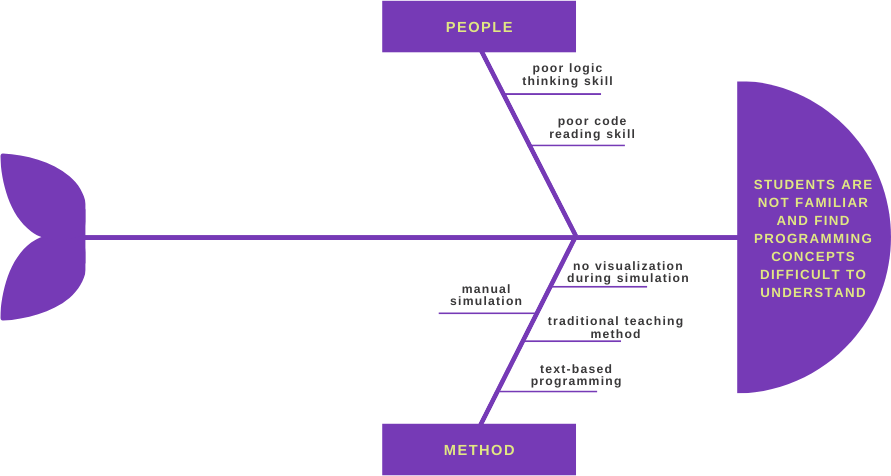
\includegraphics[width=0.8\textheight,angle=90]{figures/fishbone1.png}
			\caption[Ishikawa Diagram 1]{Fishbone diagram of the students are not familiar and find
			programming concepts difficult to understand}
			\label{fig:fishbone1}
		\end{figure}
		\vfill

		\newpage
		\null\vfill
		\begin{figure}[H]
			\centering
			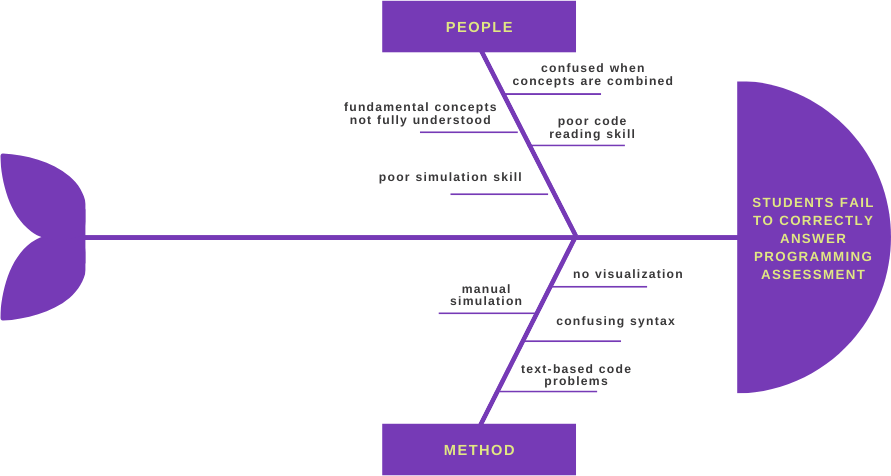
\includegraphics[width=0.8\textheight,angle=90]{figures/fishbone2.png}
			\caption[Ishikawa Diagram 2]{Fishbone diagram of the students fail to correctly answer programming
			assessment}
			\label{fig:fishbone2}
		\end{figure}
		\vfill

		\newpage
		\null\vfill
		\begin{figure}[H]
			\centering
			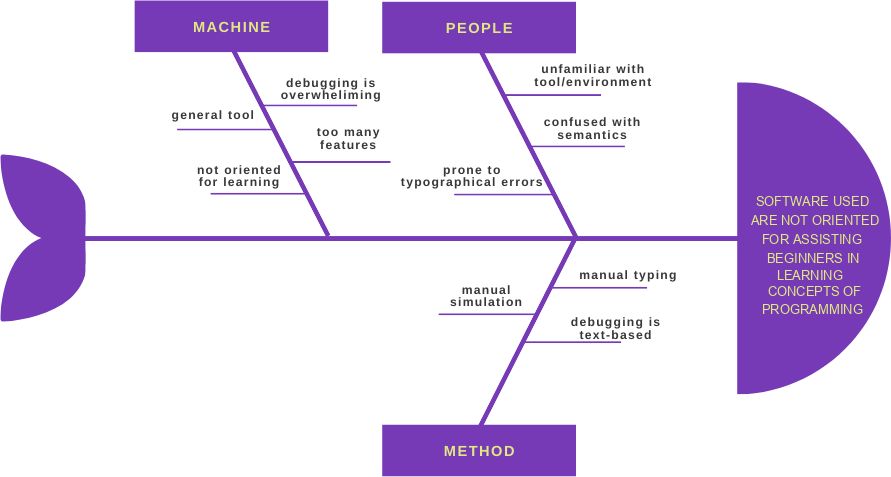
\includegraphics[width=0.8\textheight,angle=90]{figures/fishbone3.png}
			\caption[Ishikawa Diagram 3]{Fishbone diagram of the tool for programming not effective for
			learning}
			\label{fig:fishbone3}
		\end{figure}
		\vfill

		% \appendix
		% \subsection*{APPENDIX D} \label{appendixc}
		% \subsubsection*{Context Diagram (Manual)} \label{contextdiagrammanual}
		\newpage
		\null\vfill
		\begin{figure}[H]
			\centering
			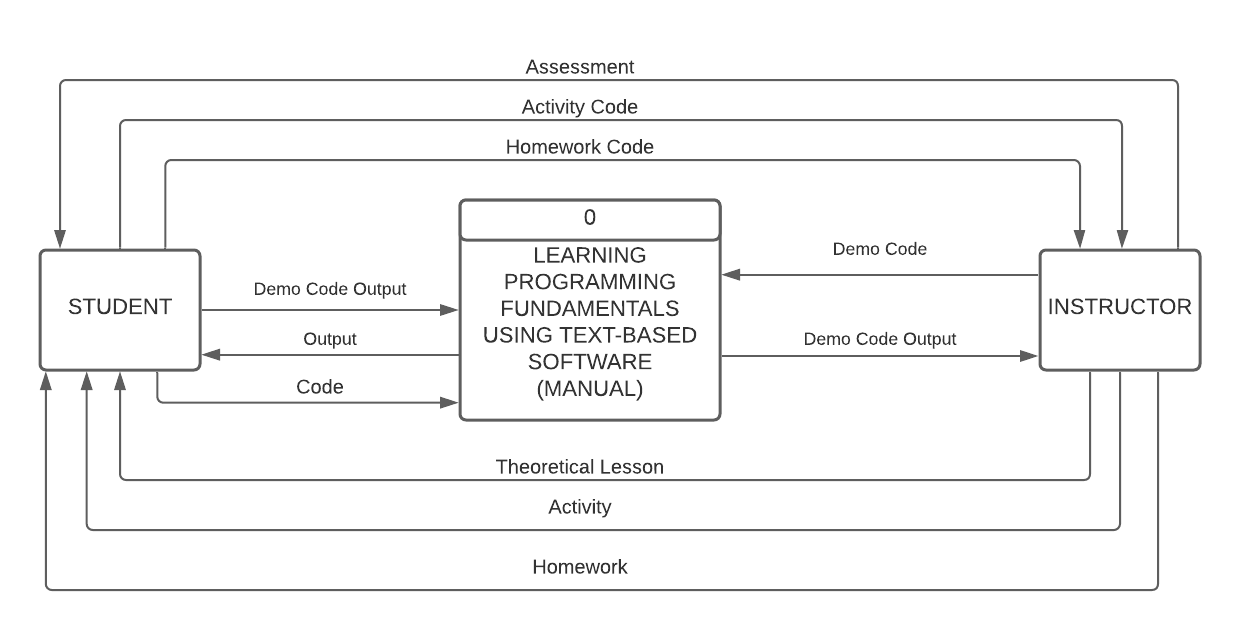
\includegraphics[width=\textwidth]{figures/context_diagram_manual.png}
			\caption{Context Diagram of Existing System}
			\label{fig:context_diagram_manual}
		\end{figure}
		\vfill

		% \subsubsection*{Context Diagram} \label{contextdiagram}
		\begin{figure}[H]
			\centering
			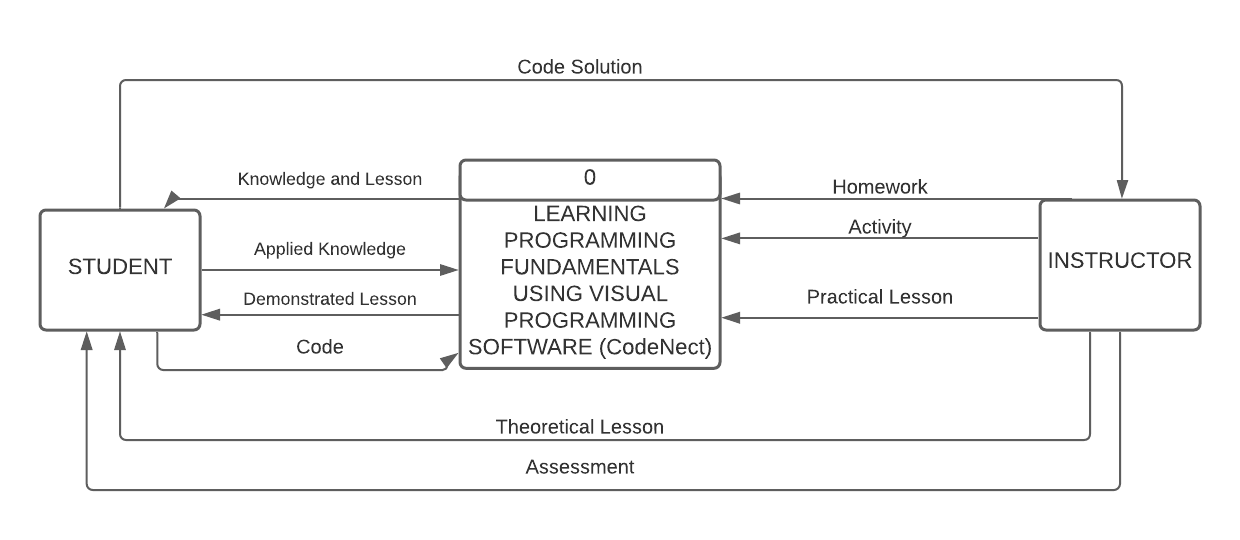
\includegraphics[width=\textwidth]{figures/context_diagram.png}
			\caption{Context Diagram of Proposed System}
			\label{fig:context_diagram}
		\end{figure}
		\vfill

		\newpage
		\null\vfill
		% \subsection*{APPENDIX E} \label{ganttchart}
		% \subsubsection*{Gantt Chart}
		\begin{figure}[H]
			\centering
			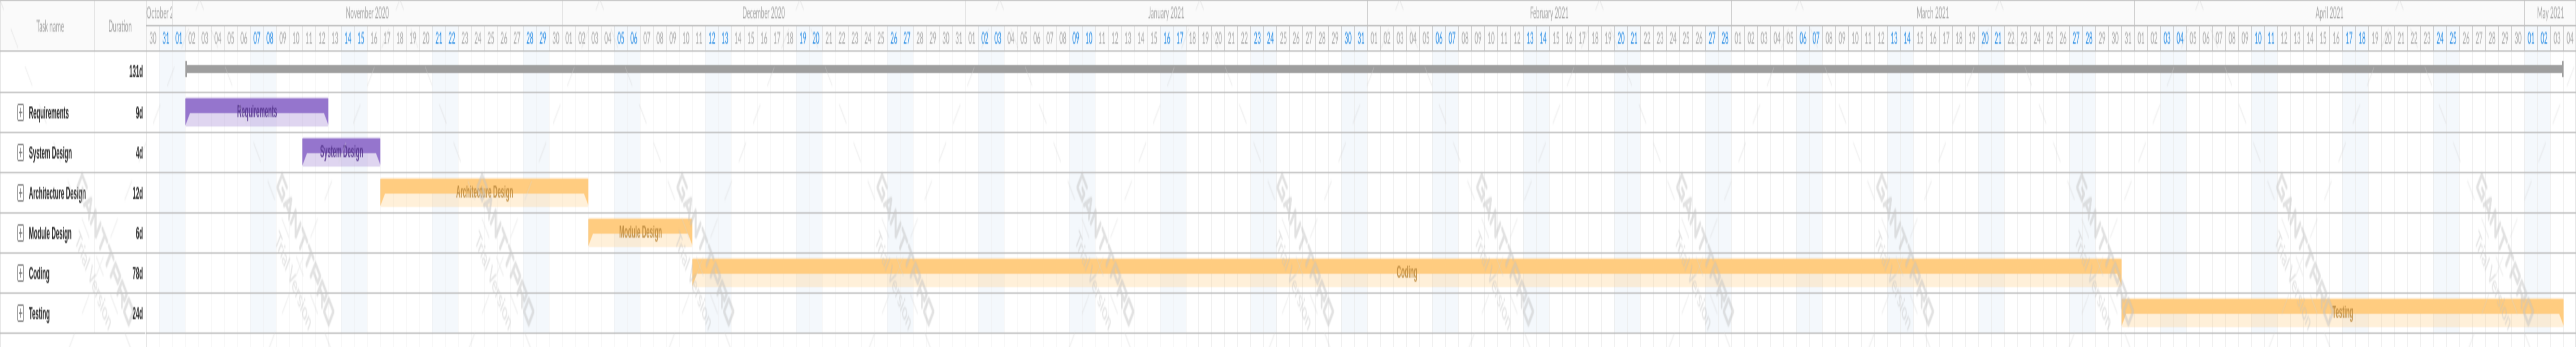
\includegraphics[width=0.8\textheight,angle=90]{figures/gantt_chart.png}
			\caption[Gantt Chart]{Gantt Chart of the Development of CodeNect}
			\label{fig:gantt_chart}
		\end{figure}
		\vfill

		\newpage
		\null\vfill
		% \subsection*{APPENDIX F} \label{theoreticalframework}
		% \subsubsection*{Theoretical Framework}
		\begin{figure}[H]
			\centering
			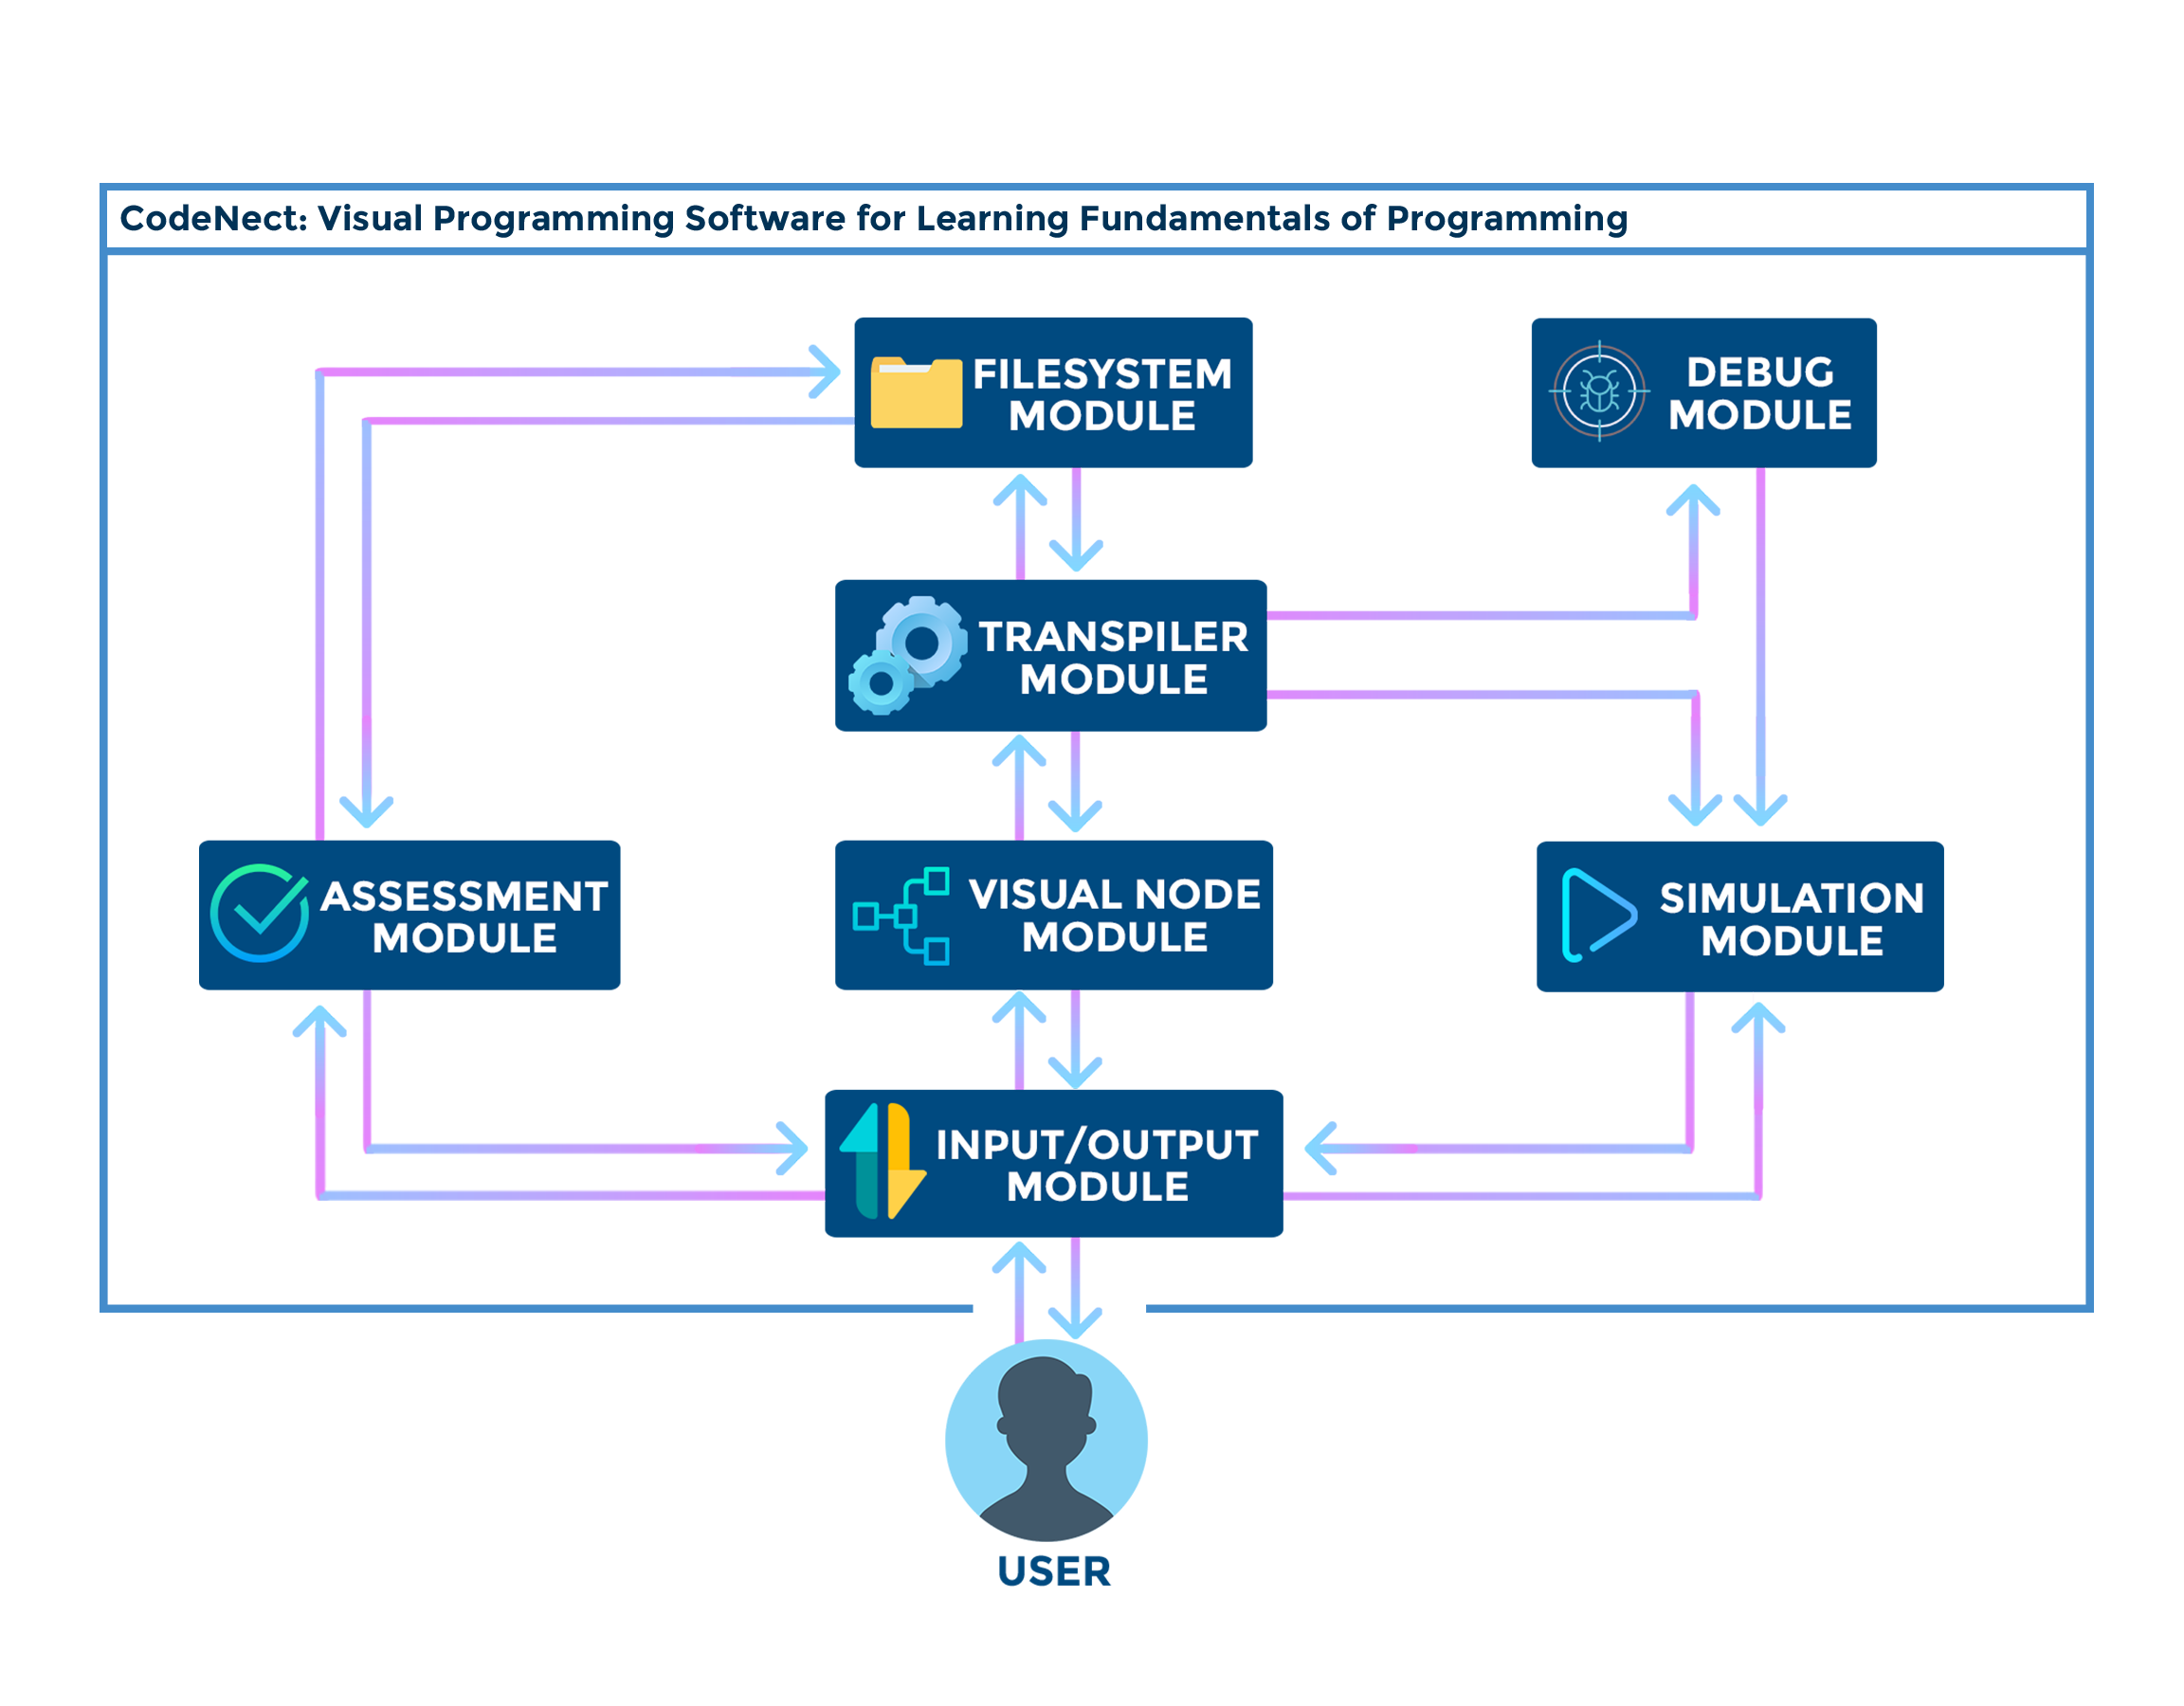
\includegraphics[width=\textwidth]{figures/theoretical_framework.png}
			\caption[Theoretical Framework]{Theoretical Framework of CodeNect: Visual Programming Software
			for Learning Fundamentals of Programming}
			\label{fig:theoretical_framework}
		\end{figure}
		\vfill

	\end{center}
\end{doublespace}
